\documentclass[11pt,usenames,dvipsnames,rgb,svgnames,x11names]{beamer} 
\usepackage{etex}
\usepackage{color}
\usepackage{xcolor}
\usetheme{Singapore}
\usepackage{amssymb,amsmath,amsthm,amsfonts}                    
\usecolortheme{dolphin} 
\setbeamertemplate{navigation symbols}{}
\usepackage[utf8]{inputenc} 
\usepackage{polski}
\usepackage{tikz}
\usepackage{tikz-qtree}
\usepackage{subfigure}
\usepackage{setspace}
\usepackage{savesym}
\savesymbol{arc}
\usepackage{pict2e}
\usepackage{epstopdf}
\usepackage{caption}
\usepackage{graphicx}
\usepackage{pict2e}
\usepackage{epstopdf}
\usepackage{geometry}
\usepackage{mathabx}
\usepackage[normalem]{ulem}
\usepackage{wrapfig}
\usepackage{multirow}
\usepackage{booktabs}
\usepackage{pifont}
% \usepackage{picins}
% \usepackage{floatflt}
%\usepackage{subcaption}
\usepackage{multirow}
\usepackage{tabularx}
\usepackage{lscape}
\usepackage{verbatim}
\usepackage{algorithm}
\usepackage{algorithmic}
\usepackage{icomma}
\usetikzlibrary{positioning}
%\usepackage[noend]{algpseudocode}
\usetikzlibrary{arrows}


\definecolor{jeden}{RGB}{255,0,0}
\definecolor{dwa}{RGB}{191,63,0}
\definecolor{trzy}{RGB}{127,127,0}
\definecolor{cztery}{RGB}{63,191,0}
\definecolor{piec}{RGB}{0, 255, 0}
\definecolor{mojkolor}{rgb}{0.99, 1, 0.99}
\definecolor{szary}{RGB}{200, 200, 200}

\title{STATYSTYCZNE METODY \newline REGRESJI PORZĄDKOWEJ}
\author{Marta Sommer}
\institute{MiNI, Politechnika Warszawska}
\titlegraphic{
\includegraphics[scale=0.5]{mini.jpg}}
\date{25 stycznia 2016r.}

\renewcommand*{\tablename}{Wykres}
\theoremstyle{plain}
\newtheorem{twierdzenie}{Twierdzenie} 
\newtheorem{twierdzeniecd}{Twierdzenie cd.} 
\theoremstyle{definition}
\newtheorem{definicja}{Definicja}
\newtheorem{przyklad}{Przykład}
\newtheorem{lemat}{Lemat}
\newtheorem{wniosek}{Wniosek}
\newtheorem{oznaczenia}{Oznaczenia}
\theoremstyle{remark}
\newtheorem{uwaga}{Uwaga}
\renewcommand*{\figurename}{Figure} 

\setbeamertemplate{caption}[numbered]
\setbeamertemplate{footline}[frame number]

\begin{document}

\begin{frame}
	\titlepage
\end{frame}

%%%%%%%%%%%%%%%%%%%%%%%%%%%%%%%%%%%%%%%%%%%%%%%%%%%%%%%%%%%%%%%%%%%%%%%%%%%%%%%%%%%%%%%%%%%%%%%%%%%%%%%%%%%%%%%%%%%%%

%\textsc{\begin{frame}
%\Huge
%\centering
%\textbf{PRZYKŁAD}
%\end{frame}

\begin{frame}
\frametitle{\textbf{MOTYWACJA}}

\begin{columns}[T]
\begin{column}{0.7\textwidth}
\centering
\textcolor{blue}{\fbox{SZUKANE}}
\end{column}

\begin{column}{0.3\textwidth}
\centering
\textcolor{blue}{\fbox{DANE}}
\end{column}
\end{columns}


\begin{columns}[T]

\begin{column}{0.3\textwidth}
\begin{center}
\textcolor{blue}{ZWYKŁA KLASYFIKACJA}
\end{center}
Czy klientowi spodoba się dana książka?
\begin{enumerate}[1)]
\item \textcolor{jeden}{nie}
\item \textcolor{piec}{tak}
\end{enumerate}
\end{column}

\begin{column}{0.4\textwidth}
\begin{center}
\textcolor{blue}{REGRESJA PORZĄDKOWA}
\end{center}
W jakim stopniu klientowi spodoba się dana książka?
\begin{enumerate}[1)]
\item \textcolor{jeden}{bardzo się nie spodoba}
\item \textcolor{dwa}{raczej się nie spodoba}
\item \textcolor{trzy}{ani się spodoba ani się nie spodoba}
\item \textcolor{cztery}{raczej się spodoba}
\item \textcolor{piec}{bardzo się spodoba}
\end{enumerate}
\end{column}
\hspace{-4mm}
\textcolor{szary}{\vrule{}}
\hspace{1mm}
\begin{column}{0.3\textwidth}
%\begin{center}
%\textcolor{white}{DANE kadsn kasdn}
%\end{center}
\vspace{1cm}
Co wiemy o kliencie?
\vspace{0.5cm}
\begin{itemize}
\item wiek
\item płeć
\item wykształcenie
\item historia zakupów
\item ...
\end{itemize}
\end{column}
  
\end{columns}  
  
\end{frame}

\begin{frame}
\frametitle{\textbf{DOSTĘPNE METODY}}
\begin{itemize}

\item model proporcjonalnych szans

$$
\log\dfrac{\mathbb{P}(Y\leq j \hspace{1mm}|\hspace{1mm} \mathbf{x})}{1-\mathbb{P}(Y\leq j \hspace{1mm}|\hspace{1mm} \mathbf{x})} = \alpha_j+\mathbf{\beta}^T\mathbf{x}
$$

\end{itemize}
\end{frame}

\begin{frame}
\begin{itemize}
\item maszyna wektorów podpierających (SVM)
\end{itemize}
\vspace{4mm}
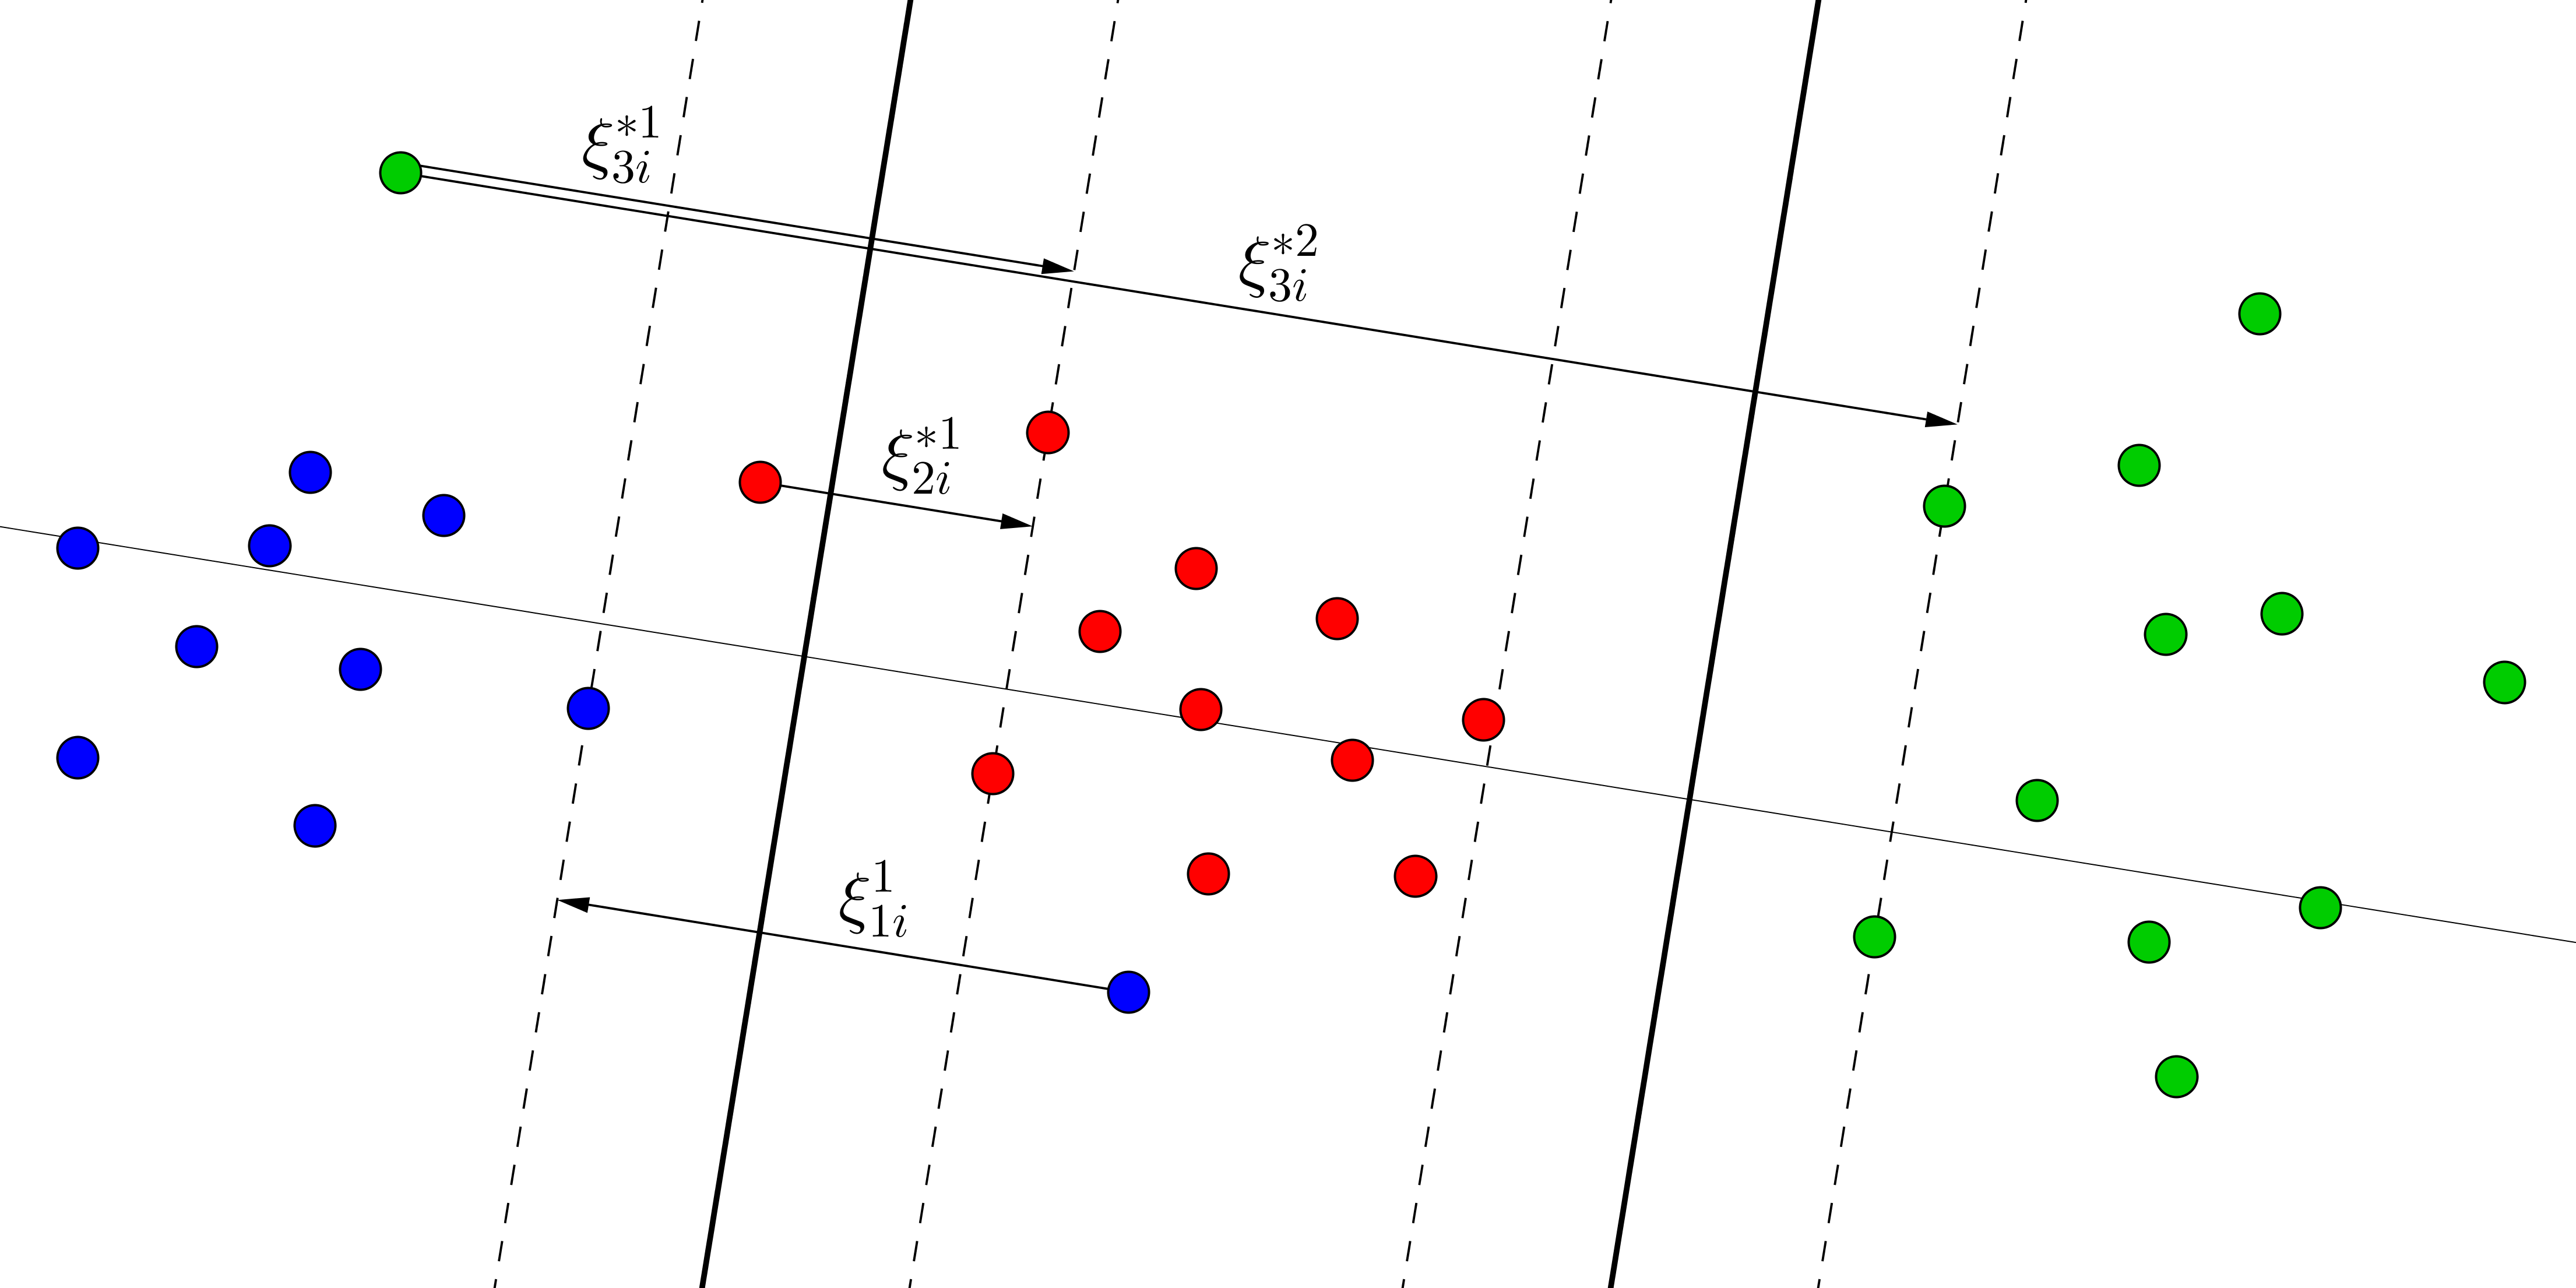
\includegraphics[scale=0.3]{svm3_dobre.png}
\end{frame}

\begin{frame}
\begin{itemize}
\item sieci neuronowe
\end{itemize}

\begin{figure}[!hb]
\begin{center}
\resizebox{0.8\textwidth}{!}{
	\def\layersep{6cm}

\begin{tikzpicture}[shorten >=1pt, ->, draw=black!50, node distance=\layersep]
    \tikzstyle{neuron}=[circle, fill=black!25, minimum size=17pt, inner sep=0pt]
    \tikzstyle{input neuron}=[neuron, fill=green!50];
    \tikzstyle{output neuron}=[neuron, fill=red!50];
    \tikzstyle{hidden neuron}=[neuron, fill=blue!50];
    \tikzstyle{annot} = [text width=5em, text centered]

    \foreach \name / \y in {1/1,K/3}
        \node[input neuron] (I-\y) at (0,-3*\y) {$\text{wejscie}^{(0)}_\name$};
    \node[draw=none, scale=4, text height=0.333cm] (I-2) at (0,-3*2) {$\vdots$};

	\foreach \name / \y in {1/1, 2/2, m/4}
        \path[yshift=1.4cm]
            node[hidden neuron] (H-\y) at (\layersep,-3*\y cm) {$\text{wyjscie}^{(1)}_{\name}$};
    \path[yshift=1.4cm]
            node[draw=none, scale=4, text height=0.333cm] (H-3) at (\layersep,-3*3 cm) {$\vdots$};

	\foreach \name / \y in {1/1, r/3}
        \path[yshift=0cm]
            node[output neuron] (O-\y) at (2*\layersep,-3*\y cm) {$\text{wyjscie}^{(2)}_{\name}$};
    \path[yshift=0cm]
            node[draw=none, scale=4, text height=0.333cm] (O-2) at (2*\layersep,-3*2 cm) {$\vdots$};

	\foreach \source / \sname in {1/1,3/K}
        \foreach \dest / \dname in {1/1,2/2,4/m}
            \path (I-\source) edge node[pos=0.25, sloped, fill=mojkolor, opacity=0.9, text opacity=1]{$w_{\sname\rightarrow\dname}^{(1)}$} (H-\dest);
    \foreach \source / \sname in {1/1,2/2,4/m}
    	\foreach \dest / \dname in {1/1,3/r}
        \path (H-\source) edge node[pos=0.75, sloped, fill=mojkolor, opacity=0.9, text opacity=1]{$w_{\sname\rightarrow\dname}^{(2)}$} (O-\dest);
        
    \node[annot,above of=H-1, node distance=1.5cm] (hl) {Warstwa ukryta};
    \node[annot,left of=hl] {Warstwa wejściowa};
    \node[annot,right of=hl] {Warstwa wyjściowa};

\end{tikzpicture}
}
\end{center}

\end{figure}

\end{frame}

\begin{frame}
\begin{itemize}
\item metoda Franka i Halla
\end{itemize}

\begin{figure}[h]
\begin{center}
\resizebox{0.85\textwidth}{!}{
	\begin{tikzpicture}
		\node(gora) {\begin{tabular}{c|c}
					$\mathbf{x}$ & $y$ \\
					[1ex] \hline \\ [-1.5ex] 
					$x_1^{(1)}$ $\ldots$ $x_K^{(1)}$ & $1$ \\
					[1ex] $x_1^{(2)}$ $\ldots$ $x_K^{(2)}$ & $5$ \\
					[1ex] $x_1^{(3)}$ $\ldots$ $x_K^{(3)}$ & $1$ \\
					[1ex] \vdots & $\vdots$ \\
					[1ex] $x_1^{(n)}$ $\ldots$ $x_K^{(n)}$ & $2$\\
				\end{tabular}};
		\node [below= 4cm of gora] (srodek) {$\ldots$};
		\node [right= 3cm of srodek] (prawo) {\begin{tabular}{c|c}
					$\mathbf{x}$ & $y^{(4)}$ \\
					[1ex] \hline \\ [-1.5ex] 
					$x_1^{(1)}$ $\ldots$ $x_K^{(1)}$ & $0$ \\
					[1ex] $x_1^{(2)}$ $\ldots$ $x_K^{(2)}$ & $1$ \\
					[1ex] $x_1^{(3)}$ $\ldots$ $x_K^{(3)}$ & $0$ \\
					[1ex] \vdots & $\vdots$ \\
					[1ex] $x_1^{(n)}$ $\ldots$ $x_K^{(n)}$ & $0$\\
				\end{tabular}};
		\node [left= 3cm of srodek] (lewo) {\begin{tabular}{c|c}
					$\mathbf{x}$ & $y^{(1)}$ \\
					[1ex] \hline \\ [-1.5ex] 
					$x_1^{(1)}$ $\ldots$ $x_K^{(1)}$ & $0$ \\
					[1ex] $x_1^{(2)}$ $\ldots$ $x_K^{(2)}$ & $1$ \\
					[1ex] $x_1^{(3)}$ $\ldots$ $x_K^{(3)}$ & $0$ \\
					[1ex] \vdots & $\vdots$ \\
					[1ex] $x_1^{(n)}$ $\ldots$ $x_K^{(n)}$ & $1$\\
				\end{tabular}};
		\path[draw, -latex',thick] (gora) -- (lewo);
		\path[draw, -latex',thick] (gora) -- (prawo);
	\end{tikzpicture}
	}
\end{center}
\end{figure}

\end{frame}



\begin{frame}
\frametitle{\textbf{DIAGNOSTYKA MODELU}}
\begin{itemize}
\item procent poprawnej klasyfikacji
\begin{equation*}
ACC = \frac{1}{n}\sum_{i=1}^n \mathbb{I}{\lbrace y_i=\hat{y}_i \rbrace}
\end{equation*}
\item średni błąd bezwzględny
\begin{equation*}
MAE = \frac{1}{n}\sum_{i=1}^n | y_i - \hat{y}_i | 
\end{equation*}
\item współczynnik VUS
\begin{equation*}
VUS = \dfrac{1}{n_1n_2\cdot\ldots\cdot n_r}\sum_{i_1=1}^{n_1}\sum_{i_2=1}^{n_2}\ldots\sum_{i_r=1}^{n_r}\mathbb{I}_{\lbrace f(\mathbf{x}_{i_1}^1)<\ldots<f(\mathbf{x}_{i_r}^r)\rbrace}
\end{equation*}
\item współczynnik BSC (oparty na sortowaniu bąbelkowym)
\end{itemize}
\end{frame}

\end{document}
